\documentclass[12pt]{article}  % default square logo

\usepackage[margin=2.8cm]{geometry}
\usepackage{setspace}
\usepackage{mathptmx} % Times font
\usepackage[utf8]{inputenc}

% handles ~ in url
\usepackage{hyperref}

% center captions
\usepackage[justification=centering]{caption}

% code listing
\usepackage{listings}
\usepackage{xcolor}

% packages for drawing
\usepackage{tikz}
\usetikzlibrary{graphs}     % create graphs

% for warning box
\usepackage{pifont,mdframed}
\usepackage{framed}

% algorithms
\usepackage[]{algorithm}
\usepackage[]{algpseudocode}



%%%%%%%%%%%%%%%%%%%%%%%%%%%%%%%%%%%%%%%%%%%%%%%%%%%%%%%%%%%%%%%%%%%%%%%%%%%%%%%%%%%%%%%%%

\onehalfspacing

%% styles for filter graph
\tikzstyle{filter} = [rectangle, draw, font=\small, text centered, rounded corners, minimum height=2em, node distance=3cm, minimum width=4em]

%% set code styles

\definecolor{dkgreen}{rgb}{0,0.6,0}
\definecolor{gray}{rgb}{0.5,0.5,0.5}
\definecolor{mauve}{rgb}{0.58,0,0.82}

\lstset{
  frame=tb,
  language=scala,
  aboveskip=3mm,
  belowskip=3mm,
  showstringspaces=false,
  columns=flexible,
  basicstyle={\small\ttfamily},
  numbers=none,
  numberstyle=\tiny\color{gray},
  keywordstyle=\color{blue},
  commentstyle=\color{dkgreen},
  stringstyle=\color{mauve},
  breaklines=true,
  breakatwhitespace=true,
  tabsize=3,
}

%% warning box

\newenvironment{warning}
               {\par\begin{mdframed}[linewidth=1pt,linecolor=red!20,backgroundcolor=yellow!40]%
                 \begin{list}{}{\leftmargin=1cm
                     \labelwidth=\leftmargin}\item[\Large\ding{43}]}
               {\end{list}\end{mdframed}\par}

\newenvironment{info}
               {\par\begin{mdframed}[linewidth=1pt,backgroundcolor=blue!20!white]%
                 \begin{list}{}{\leftmargin=1cm
                     \labelwidth=\leftmargin}\item[\Large\ding{46}]}
               {\end{list}\end{mdframed}\par}

%%%%%%%%%%%%%%%%%%%%%%%%%%%%%%%%%%%%%%%%%%%%%%%%%%%%%%%%%%%%%%%%%%%%%%%%%%%%%%%%%%%%%%%%%
\begin{document}

%!TEX root = ../guide.tex

\begin{titlepage}

  \begin{center}

    %% \vspace{20cm}
    \vspace*{3\baselineskip}
    % Title
    {\Large \bfseries Trading Simulation framework: Programming Guide\\[0.4cm] }

    % Authors and supervisor
    \noindent
    The Trading Simulation Developer Team \\[4cm]

    \begin{framed}
    Project of Big Data Course \\
    Professor: Christoph Koch \\
    Supervisor: Mohammad Dashti
    \end{framed}

    \noindent
    Lausanne, Academic Year 2014 - 2015 \\[0.3cm]

    % Upper part of the page. The '~' is needed because \\
    % only works if a paragraph has started.
    \includegraphics[width=0.2\textwidth]{img/epfl}~\\[1cm]

    \vfill

    % Bottom of the page
    {\large \today}

  \end{center}

\end{titlepage}

\subsection*{Preface}

The targeted audience of this documentation is developers who want to use the TradingSimulation framework to experiment with algorithmic trading or contribute to the TradingSimulation project. The readers should have some background in algorithmic trading or have access to expertises of the field. The reader should also be familiar with programming in Scala.


\pagenumbering{Roman}
\tableofcontents

\pagenumbering{arabic}

%!TEX root = ../guide.tex

\section{Introduction}
\label{sec:1}

This section introduces the functionalities, use cases and architecture of the TradingSimuation framework.

\subsection{What's TradingSimulation}

TradingSimulation is an open source\footnote{\url{https://github.com/merlinND/TradingSimulation}} algorithmic trading framework based on Scala\footnote{\url{http://scala-lang.org}}. The framework provides a lot of standardized components, which can be easily composed by the programmers with a few lines of Scala code to do various experiments related to algorithmic trading.

Following are a list of use cases of TradingSimulation:

\begin{itemize}
\item Simulation of multiple traders in a virtual market
\item Evaluation of a trading algorithm against live Forex data
\item Evaluation of a trading algorithm against live Bitcoin data
\item Evaluation of a trading algorithm based on historical market data
\end{itemize}

\subsection{The Architecture of TradingSimulation}

The design of TradingSimulation is based on the \emph{Pipes and Filters}\footnote{\url{http://www.cs.olemiss.edu/~hcc/csci581oo/notes/pipes.html}} architectural pattern, which results in a very high level of modularity, extensibility and reusability of the framework.

In the terminology of \emph{Pipes and Filters}, the standard components provided by the TradingSimulation framework are called \emph{filters}. The programmers can select appropriate filters and connect them properly according to the specific experiment purpose. Each configuration of filters is called a \emph{filter graph}.

Figure~\ref{fig-filter-graph} is an example filter graph of TradingSimulation. In the filter graph, there are six inter-connected filters.


\begin{figure}
  \centering
  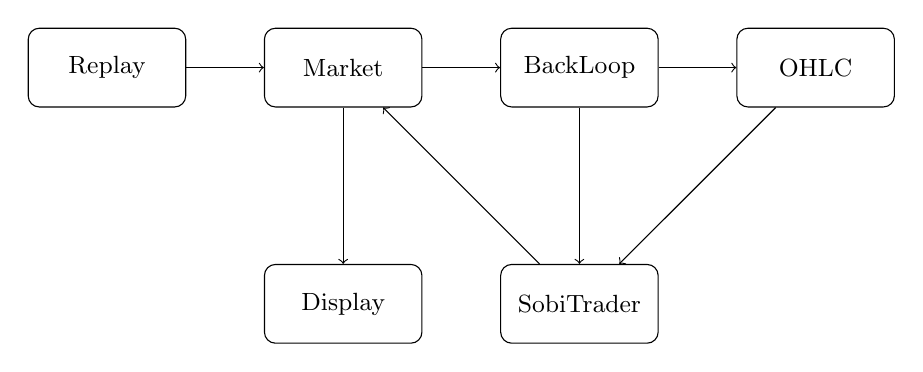
\begin{tikzpicture}[every node/.style={rectangle, draw, font=\small, text centered, rounded corners, node distance=3cm, minimum height=1cm, minimum width=2cm}]
    \node (Replay) {Replay};
    \node [right of=Replay] (Market) {Market};
    \node [right of=Market] (BackLoop) {BackLoop};
    \node [right of=BackLoop] (OHLC) {OHLC};
    \node [below of=BackLoop] (SobiTrader) {SobiTrader};
    \node [below of=Market] (Display) {Display};

    \graph [grow right=3cm] {
      (Replay) -> (Market) -> { (BackLoop) -> { (OHLC) -> (SobiTrader), (SobiTrader) }, (Display) };
      { (SobiTrader) } -> (Market);
    };
  \end{tikzpicture}
  \centering
  \caption{A Filter Graph in TradingSimulation}
  \label{fig-filter-graph}
\end{figure}

The functions of the filters in Figure~\ref{fig-filter-graph} are explained as follows:

\begin{itemize}
\item{Replay}: Read historical market order data from file system and send them one by one at a constant rate to connected filters. Replay is also called \emph{source filter}, as it doesn't have any input from other filters.
\item{Market}: Receive market orders, create transactions from matching bid and ask orders according to the configured market rules, and send transaction data to connected filters.
\item {BackLoop}: It's a utility filter, which sends everything it receives from input to output.
\item {OHLC}: It receives transaction data and send the prices of Opening, Highest, Lowest and Closing once a time in a configured interval.
\item {Display}: As its name suggests, this filter shows the data it receives in the terminal. It's also called \emph{sink filter}, as it doesn't send any data to other filters.
\item {SobiTrader}: This filter is a trader who employs the \emph{Static Order Book Imbalance}(SOBI) trading strategy. It receives market data such as orders, transactions and OHLC, and sends bid or ask orders to the \emph{Market}.
\end{itemize}

\subsection{A Simple Example}

Following code snippet is intended to give you some feel on how to create and run a filter graph in TradingSimulation.

\lstinputlisting[language=Scala]{code/simple.scala}

As you see in the code, it first creates a component builder, then uses the builder to create various  components, connects the components, and finally starts the graph.

All usages of TradingSimulation have the same form of code as shown in the code snippet, the difference lies in what components are created, what parameters are configured for components, and how components are connected.

For more and complete examples, please check our code repository here\footnote{\url{https://github.com/merlinND/TradingSimulation/tree/master/ts/src/main/scala/ch/epfl/ts/example}}.

\section{Inside Components}
\label{sec:2}

This section explains in detail how to define components, create instances of components and connect components.

\subsection{Define a Component}

In TradingSimulation, each component is an Akka\footnote{\url{http://akka.io}} actor. This can be seen from following code snippet, in which the abstract class \emph{Component} indirectly extends the trait \emph{Actor} in Akka. All concrete components extend \emph{Component}.

\begin{lstlisting}[language=Scala]
  trait Receiver extends Actor {
    def receive: PartialFunction[Any, Unit]

    def send[T: ClassTag](t: T): Unit
    def send[T: ClassTag](t: List[T]): Unit
  }

  abstract class Component extends Receiver {
    def start: Unit = {}

    def stop: Unit = {}

    def receiver: PartialFunction[Any, Unit]
  }
\end{lstlisting}

The framework defines three standard methods for every concrete component class:

\begin{itemize}
\item{start}: concrete components can override this method to do custom initialization.
\item{stop}: concrete components can override this method to release resources.
\item{receiver}: concrete components override this method to receive and handle messages.
\end{itemize}

The data transfer between different components is in the form of Akka messages. Concrete component classes have to override the method \emph{receiver} in order to handle the messages they are interested in.

To send a message, a concrete component class can call one of the two \emph{send} methods defined in \emph{Receiver}. The two \emph{send} methods have default implementation in \emph{Component}, a concrete component class should not override them.

Following code snippet illustrates a very simple component which just prints and forwards every message it receives.

\begin{lstlisting}[language=Scala]
  class BackLoop extends Component {
    override def receiver = {
      case m =>
        println(m)
        send(m)
    }
  }
\end{lstlisting}

\subsection{Create Instances of Components}

To create an instance of a component, we have to first create a \emph{component builder} as follows:

\begin{lstlisting}[language=Scala]
val builder = new ComponentBuilder("test")
\end{lstlisting}

Now suppose we have a Component \emph{OhlcIndicator} defined as follows:

\begin{lstlisting}[language=Scala]
  class OhlcIndicator(marketId: Long, symbol: (Currency,Currency), tickSizeMillis: Long) extends Component   {
    // ...
  }
\end{lstlisting}

Then we can create an instance of \emph{OhlcIndicator} with following code snippet:

\begin{lstlisting}[language=Scala]
  val props = Props(classOf[OhlcIndicator], 1L, Currency.USD -> Currency.CHF, 50)
  val ohlc = builder.createRef(props, "ohlc")
\end{lstlisting}

As you can see in the code snippet above, first we create an instance of \emph{Props}\footnote{\url{http://doc.akka.io/api/akka/2.3.1/index.html\#akka.actor.Props}}. The first argument to \emph{Props} is the class we want to instantiate, and the remaining arguments are exactly the parameters that the constructor of the class \emph{OhlcIndicator} expects.

In the second line, \emph{builder.createRef} then takes \emph{props} and a name for the component to create an instance of the component. Note that the return value of \emph{builder.createRef} is a pointer to an instance of \emph{ComponentRef} instead of \emph{OhlcIndicator}.

We have learned how to created instances of components, next let's see how to connect them.

\begin{info}
Internally, \emph{builder.createRef} will call \emph{actorOf} on an instance of \emph{ActorSystem} to create an instance of the component. The whole process seems a little awkward, but that's how Akka works. If you ever have a chance to checkout Akka(\href{http://akka.io}{akka.io}), you'll find it's worth the pain.
\end{info}

\subsection{Connect Components}

To connect an upstream component A to a downstream component B, we need to specify what types of messages B expects to receive from A. During the running A would only send messages of the specified types to B. For example, in the following code snippet, \emph{trader} will only send \emph{LimitBidOrder} messages to \emph{market}, and only send \emph{LimitAskOrder} messages to \emph{display}.

\begin{lstlisting}[language=Scala]
  trader -> (market, classOf[LimitBidOrder])
  trader -> (display, classOf[LimitAskOrder])
\end{lstlisting}

A downstream component can register as many message types as the upstream component can provide. For example, in the following code snippet \emph{trader} would send both \emph{LimitBidOrder} and \emph{LimitAskOrder} messages to \emph{market}.

\begin{lstlisting}[language=Scala]
  trader -> (market, classOf[LimitBidOrder], classOf[LimitAskOrder])
\end{lstlisting}

If a downstream component registers a message type that the upstream component can't provide, the registration has no effect. In practice, it's important to check carefully what messages a component can receive and provide.

\subsection{Traders}

Traders are basically components, but their definition and creation are more involved, so they need a special section.

In order to support automatic optimization of strategy parameters, all traders take parameters as following:

\begin{lstlisting}[language=Scala]
  class MovingAverageTrader(uid: Long, parameters: StrategyParameters) extends Trader(uid, parameters) {
    // ...
  }
\end{lstlisting}

The first parameter is the trader ID, the second parameter is a collection of parameters. There are following types of parameters:

\begin{itemize}
\item \emph{BooleanParameter}: represents boolean parameters.
\item \emph{CoefficientParameter}: represents a floating point coefficient in range [0, 1].
\item \emph{NaturalNumberParameter}: represents an integer number greater or equal to zero.
\item \emph{RealNumberParameter}: represents a real number greater than an initial value.
\item \emph{TimeParameter}: represents a duration of time.
\item \emph{CurrencyPairParameter}: represents a pair of currencies to be traded.
\item \emph{WalletParameter}: represents funds in various currencies.
\item \emph{MarketRulesParameter}: represents rules applied in a certain market.
\end{itemize}

To create an instance of a specific trader, you need to know what parameters it takes exactly. The information about parameters can be found both in code and documentation. Once you know what parameters a trader takes, you can create the \emph{StrategyParameters} object as follows:

\begin{lstlisting}[language=Scala]
  val initialFunds = Map(Currency.CHF -> 5000.0)
  val parameters = new StrategyParameters(
    MovingAverageTrader.INITIAL_FUNDS -> WalletParameter(initialFunds),
    MovingAverageTrader.SYMBOL -> CurrencyPairParameter(symbol),
    MovingAverageTrader.SHORT_PERIOD -> new TimeParameter(periods(0) seconds),
    MovingAverageTrader.LONG_PERIOD -> new TimeParameter(periods(1) seconds),
    MovingAverageTrader.TOLERANCE -> RealNumberParameter(0.0002))
\end{lstlisting}

Now, you can create the trader with just one line of code as follows:

\begin{lstlisting}[language=Scala]
  val trader = MovingAverageTrader.getInstance(10L, parameters, "MovingAverageTrader")
\end{lstlisting}

In the code above, \emph{MovingAverageTrader} is a companion object of the class \emph{MovingAverageTrader}, which provides the method \emph{getInstance} to create a new instance of the component. The method \emph{getInstance} takes a \emph{builder} as implicit parameter. Either make sure an implicit \emph{builder} is in scope or provide it explicitly.

\begin{warning}
In theory, you can also create an instance of \emph{MovingAverageTrader} like a common component as follows. But this is not recommended, as the \emph{getInstance} approach provides more safety check of parameters.

\begin{lstlisting}[language=Scala]
  val trader = builder.createRef(Props(classOf[MovingAverageTrader], 10L, parameters), "trader")
\end{lstlisting}
\end{warning}

Once created, traders can be connected exactly the same way as common components, thus it's omitted here.

Definition of new traders is more involved, which I leave to the interested reader to discover in the code base\footnote{All information about traders can be found in the package \emph{ch.epfl.ts.traders}}.

\section{Usage Scenarios}
\label{sec:3}

This section introduces in detail how to use the framework for common usage scenarios.

\subsection{Bitcoin Trading}

In this example, we demonstrate how to use the framework to experiment Bitcoin trading with the \emph{MovingAverageTrader} on live market data. The component graph of this application is as follows:

\noindent
\includegraphics[width=\textwidth]{img/examples/btce}

The BTC-E fetchers get orders and transactions from \url{btc-e.com}, feed them to the market simulator. The market simulator generates transactions based on the bid and ask orders from the trader. The trader sends bid or ask orders to the market simulator based on the transactions received from the market simulator. The printer prints information about the market in the console.

\subsection{Forex Trading}

In this example, we demonstrate how to use the framework to experiment Forex trading with the \emph{MovingAverageTrader} on live Forex data. The component graph of this application is as follows:

\noindent
\includegraphics[width=\textwidth]{img/examples/forex-live}

In the component graph above, the fetcher gets live quotes data from \url{webrates.truefx.com}, and feeds them into the market simulator, trader and broker.

The trader makes sell and buy decisions based on the quotes received from the fetcher, and send them to the broker.

The broker receives orders from the trader, and forward them into the market simulator on behalf of the trader. Note that the usage of broker is optional, it's used here only for illustrating purpose.

The market simulator generates transactions based on the orders from traders.

\subsection{Replay}

Forex or Bitcoin trading with a single trader from history data

\subsection{Simulation with Multiple Traders}

Multiple trader simulation in a virtual market.

\section{Simulation}

\subsection{Initial Parameters}
Even though our project implements essential parts of the foreign exchange 
market, many scenarios that can happen in reality cannot be modelled in out 
simulation. Given the interplay of various counterparts involved and also the
diversity of possible trading options (out of which we only implement spot transactions) make the  market an extremely complex system.

We try to simplify as much as possible by deviding the counterparts into
non-financial traders (that use our strategies) and market maker. There is 
one market maker per symbol and each trader is only trading on one symbol. 

Finding appropriate parameters to configure a simulation that reflects the
true market has become a difficult task since existing statistics focus on 
the effects of the market, meaning the daily turnover, volumes that are
traded or market share distribution. However, it seems impossible to find 
facts like "how many people are involved?" or "what are their funds?".
As such, we can find information about what results from people's trading 
activity i.e. the result of people having money to play with and be active.
However, we need to find a reasonable concept to set their initial funds to allow them being active.

- to initialize the simulation we assign money to traders and market makers in a certain currency (e.g. USD) and they receive the respective amount in the currency they need. we do it the following way:

for each symbol

1. define number of non-financial traders

2. for each trader: assign initial funds as 1-year income according to a local income distribution (e.g. Switzerland: http://www.bfs.admin.ch/bfs/portal/en/index/themen/03/04/blank/key/lohnstruktur/lohnverteilung.html)

3. compute market makers initial funds as sum(funds(all traders)) * scale

\subsection{Price Definition in Extreme Cases}

I might also have found a solution to "how is the price defined when there is nobody on the other side (offering when I want to buy or asking when I want to sell)?".
here http://www.forextraders.com/market-maker-forex-brokers.html I read that each market maker defines its own spread, which I understand the following way:

if there are only sellers and no buyers:
-  the ask price is well defined as the lowest ask offer but the bid price is not
- the market maker defines the bid price by applying its own spread to the lowest ask price
-> selling at market price means selling to the market maker for the lowest ask price MINUS the spread

if there are only buyers and no sellers:
- the bid price is well defined as the highest bid offer but the ask price is not
- again, the market maker defines the bid price by applying its own spread to the highest bid price
-> buying at market price means buying from the market maker at the highest bid price PLUS the spread

\subsection{Brain Storm}

Market Simulation Research

[1] http://www.tpc.org/tpc_documents_current_versions/pdf/tpce-v1.14.0.pdf
[2] www.swissquote.com
[3] http://vantagepointtrading.com/daily-forex-stats
[4] http://www.bis.org/publ/qtrpdf/r_qt1312e.pdf
[5] turnovers by counterparty and currency pairs:
http://www.reuters.com/article/2013/09/05/bis-survey-volumes-idUSL6N0GZ34R20130905

[6] largest forex centers:
http://countingpips.com/fx/2011/08/8-largest-forex-trading-centers-in-the-world/

[7] directional trading volume:
http://www.dailyfx.com/forex/technical/article/special_report/2015/04/13/forex-introducing-volume-by-price.html

[8] https://mahifx.com/blog/50-fascinating-facts-about-forex

[9] largest brokers by volume:
http://www.myfxbook.com/forex-broker-volume

[10] volume survey (North America) with explanation
http://www.newyorkfed.org/fxc/volumesurvey/explanatory_notes.html

[11] forex glossary
http://www.cmsfx.com/en/forex-education/Forex-Glossary/ask-price/

[12] salary distribution switzerland
http://www.bfs.admin.ch/bfs/portal/en/index/themen/03/04/blank/key/lohnstruktur/lohnverteilung.html

[13] explanation of market makers
http://www.forextraders.com/market-maker-forex-brokers.html

p.47 
- Entity Relationships
- Trade Types
- run historical data for 300 business days before simulation starts

Wanted:
- trader initial funds -> half of annual income according to [12]?
- broker initial funds (for leverage trades)
- market maker funds
- number of traders per currency pair
- one market maker per currency pair?

Assumptions:
1. all traders come from the same country
    -> initial funds are distributed according to the local wealth distribution

    2. number of traders trading a particular symbol reflects [10]

    Configuration:
    country:    Switzerland, 5th largest forex center (in 2011), Average Daily Trading Volume: \$263 billion, Percentage of Daily Global Forex Volume: 5 \%
    for each symbol
    1. define number of non-financial traders
    2. assign initial funds to each trader according to [12] equivalent to 1-year income
    3. compute market makers initial funds as sum(funds(all traders)) * scale


    counterparties: pool of non-financial customers, 1 market maker

    instruments:    only spot transactions


\end{document}
